% Capítulo 4
\chapter{Taxonomia}
\label{cap:cap4}

Prosseguindo a análise dos trabalhos mencionados no Capítulo \ref{cap:cap3}, verifica-se a necessidade de classificar dos conceitos mais recorrentes atrelados ao uso do padrão \textit{throttling} aos dispositivos em computação dirigida à energia. Além disso, é preciso levar em consideração a orientação do trabalho junto aos critérios de dependabilidade, especialmente ao concentrar-se sobre o atributo disponibilidade, elemento participante nos critérios apresentados na taxonomia proposta por \citeauthor{avizienis_basic_2004} (\citeyear{avizienis_basic_2004}). Por definição,  disponibilidade é um indicador da capacidade de um equipamento, sistema ou serviço estar em um estado que possa desempenhar certa função solicitada quando necessário \cite{ISO9000}. 

\section{Organização}

As classes descritas foram categorizadas para acomodar os elementos envolvidos de acordo com os critérios que representam. À esquerda, apresenta-se as características dos dispositivos \acs{IoT} encontrados em cenários de restrições energéticas. Primeiramente, as classes foram projetadas para organizar os elementos em destaque considerando as especificidades e limitações à operar em ambientes com recursos energéticos limitados. Estes critérios, auxiliam na compreensão mais precisa em relação as categorias e necessidades dos dispositivos e justificam o interesse sobre ações que aumentem sua disponibilidade enquanto manter suas capacidades energéticoas. Assim, os elementos participantes da taxonomia podem ser visualizados na Figura \ref{fig:cap4divisaobasetaxonomia}. 

%agentes
Enquanto ao fator que caracteriza um agente, \citeonline{avizienis_basic_2004} aplica a dinâmica de definição enquanto papéis, proporcionando clara divisão entre agentes em referencia ao que desempenha em relação ao ambiente inserido. Sendo assim, são propostos dois grupos: os clientes, que atuam ativamente realizando solicitações ou de forma passiva operam sobre  eventos realizados;  um segundo grupo, os provedores, para estes cabe a responsabilidade de compartilhar seus recursos com outros consumidores através de uma interface conhecida, de acordo com protocolo pré-estabelecido entre as partes.

%Operaçoes
Toda interação segue um padrão denominado operação, esta é realizada de acordo com o qual se destina, como visto no trabalho de \cite{khairnar_discrete-rate_2015} operações podem ser medidas pela quantidade de mensagens trocadas entre dispositivos contribuindo para um determinado fim. Representam operações, o conjunto de atividades solititadas e atendidas durante os ciclos de operação dos dispositivos. Sendo assim, os elementos classificadores foram: \textit{Agentes}, \textit{Recursos} e \textit{Operações}.

%recursos
Além disso, identificou-se a necessidade de classificar as características energéticas dos elementos participantes, uma vez que os agentes dependem ativamente de algum fator energéticos para exercer suas capacidades. Portanto, os recursos energéticos emergem como uma classe fundamental de análise para tomada de decisão sobre a aplicação dos mecanismos de limitação dos ciclos.


\begin{figure}[hbt]
	\centering
	\caption{Divisão Base da Taxonomia}
	\label{fig:cap4divisaobasetaxonomia}
	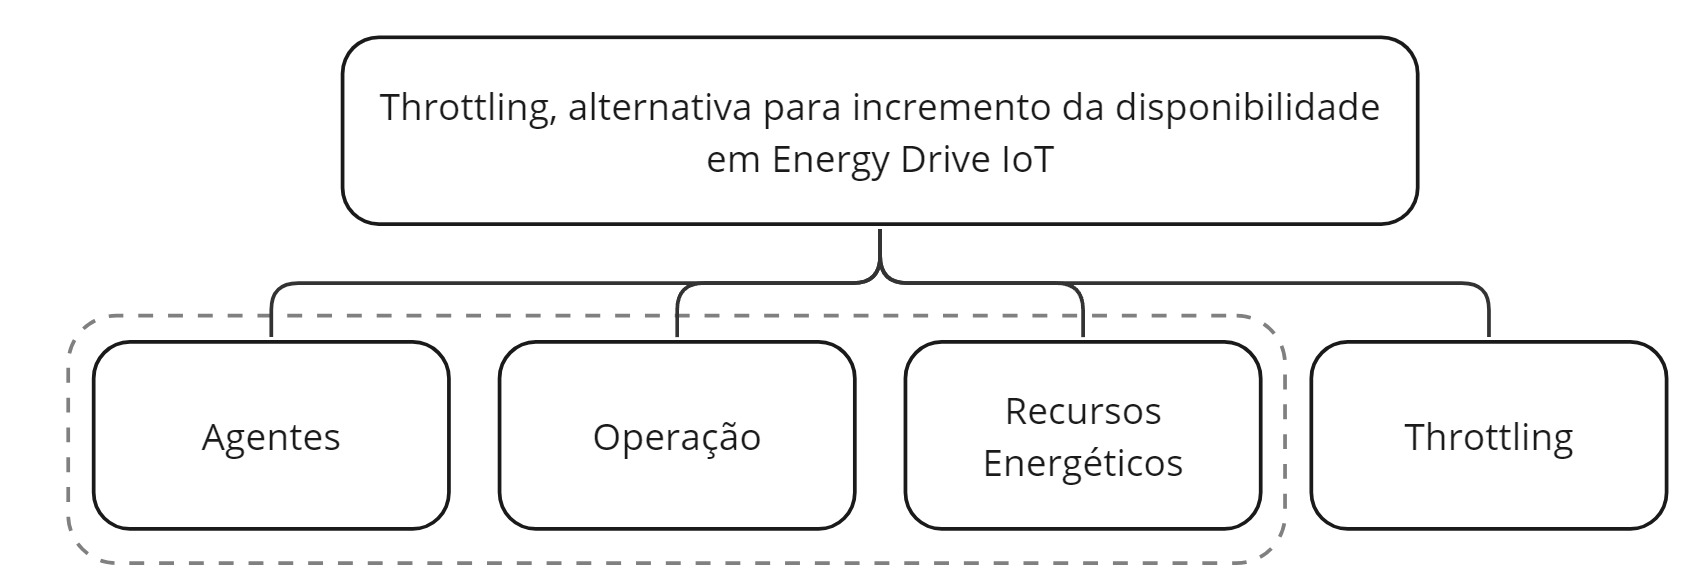
\includegraphics[width=0.7\linewidth]{Imagens/cap4/cap4taxonomia_primeironivel.jpg}	
	
	Fonte: elaborado pelo autor.
\end{figure}

Além disso, acomodam-se os elementos envolvidos no processo de gestão do comportamento de um dispositivo através do padrão \textit{Throttling}. Nesta classe, dois ramos principais são derivados: quanto a atuação e motivadores, respectivamente. A classe Atuação engloba os elementos relacionados ao processo de ajuste de comportamento, incluindo Limiar (\textit{Thresholding}), Ciclos, Meios e Observáveis. Por fim, a classe Motivação é sugerida para declarar as intenções encontradas enquanto o dispositivo busca o incremento de disponibilidade. 

\begin{figure}[hbt]
	\centering
	\caption{Visão Geral da Taxonomia.}
	\label{fig:visaogeraltaxonomia}
	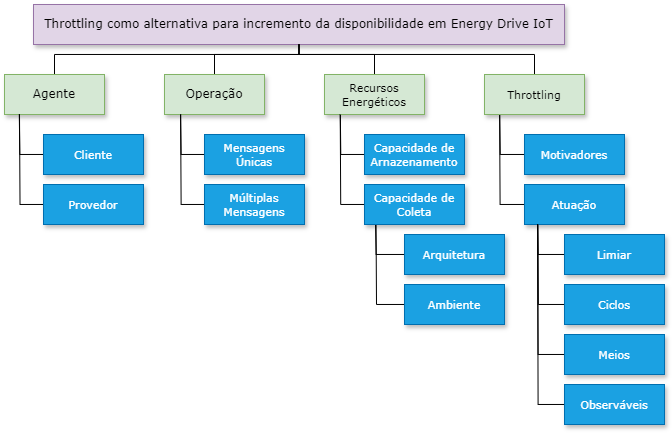
\includegraphics[width=\textwidth]{Imagens/anexos/anexo_visaogeraltaxonomia.png}	
	
	Fonte: elaborado pelo autor.
\end{figure}

\section{Taxonomia Proposta}

A Figura \ref{fig:visaogeraltaxonomia} apresenta a taxonomia com os pontos abordados na observação dos aspectos relacionados ao uso do padrão \textit{Throttling} como alternativa para garantir disponibilidade nos agentes \acs{IoT}. O principal objetivo é dispor visualmente os elementos relacionados ao tema e contemplar a organização dos tópicos envolvidos. Com isso, busca-se compreender os objetivos ao criar a taxonomia:

\begin{enumerate}
    \item Auxiliar a compreensão dos conceitos relacionados ao escopo que se define um agente \acs{IoT} em computação dirigida à energia e como o padrão \textit{Throttling} atua como agente colaborador no processo de ajuste de características nos ciclos;
  	\item Oferecer suporte às definições necessárias para uso do padrão \textit{Throttling} ligados ao contexto \acs{IoT} da computação dirigida à energia;
  	\item Facilitar a descoberta das relações entre os elementos do campo de análise.
\end{enumerate}

\section{Agentes \acs{IoT}}
Cada agente é essencialmente uma entidade que tem a capacidade intrínseca de interagir com outros agentes sejam digitais ou físicos, os chamados dispositivos. Eles possuem propriedades fundamentais, funcionalidade, desempenho e outras já definidas por \citeonline{avizienis_basic_2004}. No contexto \acs{IoT}, é crucial considerar a capacidade de se comunicar com outras entidades, além do compartilhamento de recursos \cite{asghari_internet_2019}, características intrínsecas nos dispositivos analisados.


\subsection{Dispositivo Provedor}

Em qualquer instância onde um dispositivo oferece estados ou atende solicitações de recurso, assume o papel de provedor. Para isso, o dispositivo dispõe uma ou mais funcionalidades denominadas operações, sendo cada uma, realizada através do uso de seus recursos a medida que avança em seus estados internos buscando atender as solicitações. O resultado deste processo pode ser percebido como estado externo caso necessário, acessível por meio de interface em resposta às solicitações ou provida na forma de eventos acessíveis aos clientes. 


À medida que as solicitações são recebidas pelo dispositivo provedor durante os ciclos, isso influencia diretamente na forma como ele lida com seus recursos. Essas solicitações motivam a dinâmica de mudanças de estado internas e, consequentemente, têm um impacto direto nos custos operacionais do dispositivo ao longo dos ciclos. Por exemplo, considere um sistema de iluminação urbana que interage com dispositivos em um ambiente por meio de solicitações. Esse sistema pode enviar solicitações aos dispositivos para mudar de estado e ativar um recurso em resposta a um evento específico. No caso, essa ação afetará o uso dos componentes necessários devido ao atendimento das solicitações durante ciclos, impactando assim na forma como o provedor utilizou seus recursos.


\subsection{Dispositivo Cliente}
Um dispositivo cliente é um agente físico responsável por receber o estado externo de dispositivos provedores por meio de interface disponibilizada. Ele pode consumir recursos provenientes de um ou mais provedores, dependendo da operação que precisar cumprir. De modo ativo, cabe ao cliente comunicar-se com os provedores necessários por meio de solicitações para atender suas operações. No entanto, em um caso reativo, um cliente pode permanecer inativo enquanto aguarda um evento necessário para, mediante estímulo, ativar-se com o objetivo de realizar alguma operação.


\section{Operações}
Operações consistem no fluxo de mensagens comunicáveis trocadas entre agentes clientes e provedores. Uma operação pode ser realizada quando um cliente solicita o estado de um provedor por meio de mensagens, ou quando um provedor ativamente disponibiliza um estado. É preciso destacar também que operações podem ocorrer em contexto estrito ao próprio  dispositivo, neste caso o estimulo de atuação é interno e neste ponto o dispositivo estará atendendo solicitações para si mesmo, caracterizando cliente e provedor da solicitação.

Mensagem é uma unidade atômica de informação utilizada para as mais diversas ações de acordo com o objetivo da colaboração entre dispositivos, uma mensagem pode carregar ações como inicialização, controle, monitoramento, coleta, processamento ou armazenamento de dados. Os dispositivos envolvidos devem ser capazes de interpreta-las mutualmente. Para uma operação, múltiplas mensagens também podem ser solicitadas, constituindo a composição de serviço \citeonline{kahloul_service_2019}, nesse cenário um dispositivo cliente executa solicitações distintas à um ou vários dispositivos provedores para compor sua operação. Assim definido, uma mensagem carrega em si o papel relativo à solicitação. 



\section{Recursos Energéticos}

Um recurso descreve um componente ou capacidade utilizada de tal forma que possibilita dispositivos à realizar suas operações. Isto inclui seus componentes físicos ou virtuais que uma vez embarcados ao dispositivo contribuem cooperando para os mais diversos fins, coleta, monitoramento, automação industrial, assistência a medicina entre outros. Recursos sinalizam as capacidades dos dispositivos \acs{IoT}, assim configuração dos recursos embarcados dispositivo esta fortemente ligado à atividade que se destina. 

Como observado na revisão apresentada no Capitulo \ref{cap:cap3}, e para o objetivo de categorização prevista na taxonomia, as características como capacidade de processamento, armazenamento de dados ou suas particularidades quanto sensores e componentes embarcados são omitidos pois expressam diretamente a diversidade de possibilidades ligadas o universo de atuação do dispositivo. Entretanto, os aspectos energéticos estão recorrentemente presentes a medida que se reduz o universo de análise para a computação dirigida à energia e portanto justificam seu detalhamento mediante desafios naturalmente abordados. Logo, os recursos energéticos, por sua vez refere-se aos grupos: da capacidade de coleta do dispositivo; da capacidade de armazenamento dessa energia previamente coletada. Descritos conforme abordado no portfólio de estudos criado para o estudo. 

A arquitetura dos dispositivos dirigidos a energia com capacidade de coleta são projetados para usar seus recursos energéticos de maneira eficiente \cite{prauzek_energy_2018}, sua aplicação é especialmente útil em cenários onde a energia para alimentar os dispositivos é escassa ou o fornecimento energético é inviável. Um recurso energético é propriamente uma fonte natural ou artificial de energia que pode ser convertida em forma utilizável destinada à cobrir as demandas energéticas para que o dispositivo permaneça operacional \cite{kansal_power_2007}.

No cenário proposto, observar as classes dos recursos energéticos assume um papel importante pois é essencial para garantir o funcionamento continuo e autônomo dos dispositivos envolvidos, cabendo ao dispositivo as ações de coleta, e armazenamento para posterior utilização do recurso energético, além de alguns casos, o compartilhamento desses recursos obtidos, projetando de maneira a capacitar o contexto \acs{IoT} a operar enquanto busca um cenário minimamente sustentável e caso impossibilitado, conseguir preserva-se de maneira a recupera-se em momento oportuno, restabelecidas as restrições impostas.

\subsection{Capacidade de Coleta}
\label{Capacidade de Coleta}
De acordo com \citeonline{sudevalayam_energy_2011}, a capacidade de coleta refere-se à habilidade do elemento em extrair e transformar um recurso energético disponível no ambiente. Seu objetivo é manter ou estender o tempo de funcionamento do dispositivo, atendendo integralmente ou parcialmente às suas necessidades energéticas.

Sistemas de coleta energética possuem três conceitos fundamentais: Carga, a Arquitetura de Coleta e entrada energética. A carga é destinada a atividade que, em ciclos, esta consumindo energia, este é oriundo de um componente demandante de energia no dispositivo necessário para realizar uma operação, sejam sensores, transmissores ou  atuadores. A Arquitetura de Coleta descreve quais mecanismos envolvidos, seus componentes, meios para conversão e unidades para armazenamento. Os modelos arquiteturais são fundamentados em duas propostas recorrentes, e representam características dos dispositivos oportunas para auxiliar no processo de adequação do seu gasto energético, são elas:

\begin{itemize}
    \item Coleta e Usa (\textit{Harvest-Use}): Neste modelo, toda energia coletada é oferecida diretamente ao dispositivo. Conforme \citeonline{merrett_energy-driven_2017}, um dispositivo com capacidade de coleta energética pode ser concebido de tal forma que não necessite de um armazenamento energético para suplementar operações, desde que seu funcionamento esteja orientado para abordagem neutra-potencia (\acl{PNO}). Assim, a energia coletada deve satisfazer os valores de operação plena ou pelo menos o minimo necessário para funcionamento depreciado.
        
     Outra possibilidade é apresentada em modo de operação intermitente (\acl{ICS}), onde dentre outras estratégias, permitem o dispositivo deve armazenar incrementalmente seu ultimo estado (\textit{checkpoint}) para que dada paralisação no fornecimento energético e posterior restabelecimento, o mesmo consiga retornar ao estado prévio antes da iminente interrupção. 
        
    \item Coleta, Armazena e Usa (\textit{Harvest-Store Use}): Além da coleta, busca capacitar os dispositivos de modo à armazenar a energia coletada em um componente de armazenamento, permitindo que ela seja utilizada suplementarmente nos ciclos do dispositivo caso necessário ou como fonte principal. Esse modelo visa reduzir problemas decorrentes da variação no fornecimento de energia, seja devido à escassez momentânea de energia disponível, a variação constante dos valores coletados ou à depreciação na performance do sistema de coleta.
    
\end{itemize}

A adequação da estratégia de coleta e seus detalhes devem ser projetados de acordo com o ambiente e a natureza da fonte energética que se pretende coletar. Em geral, \cite{shaikh_energy_2016} apresenta uma divisão das características das fontes energéticas, sendo sua natureza um fator primordial para que o dispositivo possa adequar seu funcionamento ao contexto encontrado. Esse aspecto pode orientar a decisão sobre permanecer ou alternar estados de funcionamento. Assim, para descrever as características dos tipos de fontes energéticas, é possível utilizar a classificação a seguir:

\begin{itemize}

    \item Não controladas mas previsíveis: A produção energética não pode ser controlada, mas seu comportamento pode ser modelado com o objetivo de prever sua disponibilidade em dado momento com alguma margem de acerto. Por exemplo, o trabalho  \cite{lee_energy_2018} aborda a gestão da gestão de recursos energéticos em dispositivos alimentados via energia solar através de análise da previsibilidade de oferta (\textit{energy forecasting}).
    
    
    \item Não controladas e não previsíveis: A fonte energética não pode ser controlada para gerar energia quando desejado e não é fácil alcançar previsibilidade para quando a oferta energética ocorrerá. A extração energética originada pela vibração de ambientes internos é um exemplo das características dessas fontes descrito em \cite{wei_comprehensive_2017} uma vez que definir padrões de sazonalidade das vibrações pode tornar o processo de coleta impraticável;
    
    \item Completamente controlada: Neste contexto, a energia é gerada apenas quando necessário, como visto em alguns sistemas que extraem energia \textit{piezoelétrico} através da interação humana para suprir necessidade energética quando oportuno.
    
    \item Parcialmente controlada: O processo de geração energética é sensível à ação de terceiros porém a quantidade exata de energia gerada não pode ser prevista com exatidão. Fontes baseadas em Radio Frequência converte a transmissão de ondas de radio em energia utilizável, por exemplo, na dinâmica realizada em tags \acf{RFID} que conseguem ser visualizadas por um leitor mediante a oferta energética provida pela antena e capturada pelo dispositivo. Todavia, a quantidade de energia coletada sofre impactos diretos das características de propagação no meio disposto, barreiras, distancia até a fonte originária, capacidade de transmissão.
\end{itemize}

\subsection{Capacidade de Armazenamento}
\label{Capacidade de Armazenamento}
A capacidade de armazenamento trata das propriedades como conversão, taxa de carregamento e descarga além de eventuais perdas em relação a fonte energética nas soluções encontradas. Seu objetivo é utilizar esse valor armazenado como suplemento energético em  momento apropriado. 

É bem conhecido que fatores energéticos representam desafios para dispositivos com restrições energéticas \cite{kansal_power_2007}, primariamente caso o recurso energético seja esgotado não será capaz de cumprir seu papel, sob a condição do inatividade até restabelecimento deste recurso ou a presença de algum mecanismo de armazenamento presente seja capaz de atender parcial ou totalmente a diferença energética necessária para as operações.  

Assim a capacidade de atuação do dispositivo buscará primariamente estar de acordo com as condições e necessidade de conservação da energia a medida que faz uso de recursos armazenados em um componente \textit{Storage}. Um acordo de nível de serviço (\acl{SLA}) de disponibilidade é fundamental para decidir e optar sobre a presença e as características desse \textit{Storage}. Portanto, quanto a capacidade de armazenamento energético um dispositivo deve encontrar-se como: 

\begin{itemize}
    \item Dispositivo sem \textit{Storage}: Aqui não existe a necessidade estrita da gestão de recursos elétricos armazenados pois caso não exista energia suficiente o dispositivo poderá adaptar-se continuamente na tentativa de manter sua necessidade energética em acordo ao fornecido no momento, ou encerrar suas operações por interrupção por valor coletado insuficiente. Neste caso é fundamental que o dispositivo esteja ciente das caracteristicas energéticas do ambiente onde está inserido.
    
    \item Dispositivo com \textit{Storage}: Neste caso, um dispositivo carrega em si a capacidade de armazenar energia coletada em um \textit{buffer}. A gestão energética deve ocorrer para que a energia coletada seja previamente armazenada e assim, disponibilizada a medida que os ciclos de funcionamento decorrem. Os dispositivos operam em um regime de Coleta, Armazenamento e Uso e não necessariamente adotam um comportamento em decorrencia do comportamento exclusivo dos valores coletados. Ao equipar dispositivos com \textit{Storage} pontos como custo, volume, capacidade desse componente e as questões ambientais em decorrencia disso devem ser ponderados conforme mecionado por \citeauthor{merrett_energy-driven_2017}(\citeyear{merrett_energy-driven_2017}).

\end{itemize}

\section{\textit{Throttling}}

O padrão \textit{Throttling} consiste basicamente em ações que buscam restringir o uso de recursos de acordo com limiares de utilização estabelecidos. Seu objetivo primário é proteger um dispositivo contra um estado de sobrecarga de atividades, evitando que consumidores excessivamente solicitantes coloquem um dispositivo em estado critico, e assim evitando possíveis falhas ou a exaustão prematura de recursos \cite{martinekuan_throttling_nodate}. Com isso, os dispositivos \acs{IoT} com restrições energéticas implementam tal mecanismo com a intenção de manter-se operando dentro de termos definidos por um acordo de funcionamento, evitando que se encontre em situação onde precise atender mais solicitações do que o adequado para sua capacidade seja computacional e mais especificamente energética.

Na taxonomia, o \textit{Throttling} é sugerido como colaborador recorrentemente presente nas atividades que buscam preservar disponibilidade dos dispositivos, conservando recursos energéticos em observação das características ou limitações do próprio dispositivo. Para tal, é da natureza do mecanismo a necessidade da definição de limiares estritamente adequados, seja sobre sua capacidade de atender solicitações, recursos coletados, disponíveis ou mesmo previstos pelo dispositivo. Definir limiares de operação realísticos que atendam as necessidades de um dispositivo provedor é um desafio para sistemas com estratégia de coleta de energia \cite{khairnar_discrete-rate_2015}, \cite{liu_energy_2016} e \cite{zhang_toward_2018}, pois entrega capacidade de decisão sobre as atividades realizadas nos ciclos enquanto objetifica permanecer energeticamente viável.

\subsection{Atuação}
\label{cap4:atuação}

\begin{figure}[hbt]
	\centering
	\caption{Throttling:Atuação.}
	\label{fig:taxonomia_atuacao}
	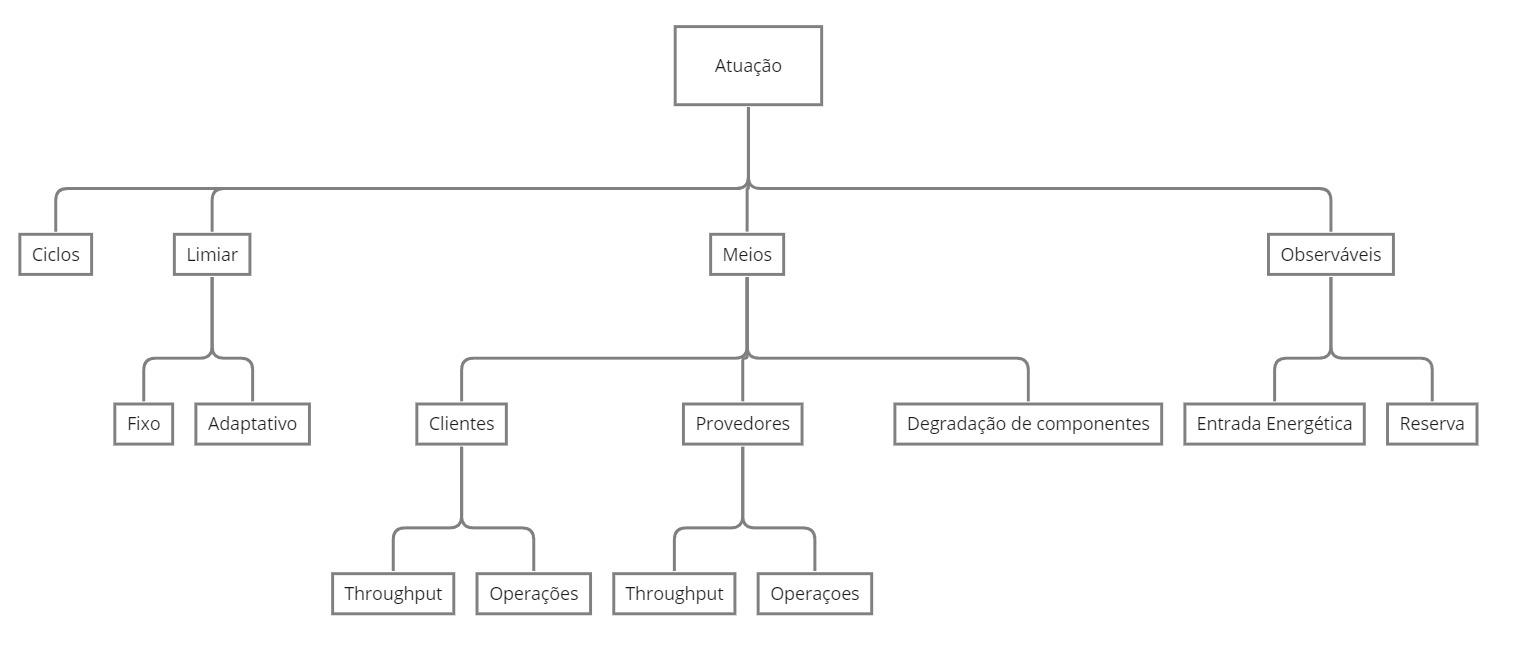
\includegraphics[width=1\textwidth]{Imagens/cap4/cap4taxonomia_throttling_atuacao.jpg}	
	
	Fonte: elaborado pelo autor.
\end{figure}

Dispositivos \acs{IoT} presentes na computação dirigida à energia, a atuação do mecanismo \textit{throttling} é dada ao sugerir como o dispositivo irá se comportar durante uma janela temporal de operações denominada Ciclo e esta disposto como categoria mais à esquerda no recorte disponível na Figura \ref{fig:taxonomia_atuacao}. Os ciclos são divisões fundamentais, sua definição foi dada por \citeonline{kansal_power_2007} e relata sobre os eventos desencadeados durante a operação do dispositivo. Durante um ciclo, clientes e provedores realizam suas atividades, solicitando e disponibilizando seus estados. Do ponto de vista da disponibilização dos recursos, durante um ciclo, um dispositivo provedor configurado para tal, pode assumir abordagem de equidade entre os solicitantes ou outro critério de prioridade e privilégio, por exemplo as características ligadas aos fatores de transmissão como encontrado em \citeonline{abrardo_game_2013}. Em virtude disso, caso seja necessário, um solicitante qualquer teria suas solicitações atendidas enquanto ocorre a negação do serviço para outro cliente com menor prioridade. Essa prática é comum em sistemas que implementam políticas de priorização, garantindo que solicitações de dispositivos com maior importância sejam atendidas antes das de menor prioridade - ou até de si próprio. Isso permite uma gestão mais eficiente dos recursos e uma melhor adaptação às demandas variáveis do ambiente.

O \textit{Throttling} utiliza mecanismos limitadores, atua baseado em limiares, através da restrição no atendimento de solicitações. Uma vez definido atuação, a ação do limitador poderá ser constante durante todo funcionamento do dispositivo, assim o mesmo valor limiar é aplicado independente de outros fatores durante todo o tempo. Outra possibilidade é definir vários limiares que agem de maneira adaptativa de acordo com os modos de operação mapeados, tão logo determinado cenário seja alcançado, o dispositivo pode ajustar seu limiar de atuação para conservar seus recursos visando manter-se funcional. O comportamento do limiar de atuação passa pela analise cuidadosa da natureza da realizacão das operações esperadas para o dispositivo e possui influencia sobre como o dispositivo irá se comportar. Quanto aos limiares, são classificados  como:

O \textit{throttling} utiliza mecanismos limitadores que atuam com base em limiares restringindo o atendimento de solicitações. Este limiar é uma indicação de que alguma ação deverá ser tomada a partir daquele instante. Uma vez definida, o valor de limiar pode ser constante ao longo de todo o funcionamento do dispositivo. Outra possibilidade é a definição de vários limiares que atuam de forma adaptativa de acordo com os modos de operação mapeados em um acordo de qualidade de serviço (\ac{QoS}) presente nos termos de funcionamento daquele dispositivo. Assim que determinado limiar é alcançado, o dispositivo pode ajustar sua atuação de acordo com o objetivo proposto. O comportamento do limiar de atuação é cuidadosamente analisado e observa sobre as capacidades energéticas dos dispositivos com base na natureza das operações esperadas para o dispositivo \acs{IoT} influenciando diretamente em seu comportamento. Quanto a dinâmica dos limiares, eles podem ser classificados como:

\begin{itemize}
    \item Limiar constante: Seu valor é fixado e estabelecido enquanto o dispositivo é projetado. Este limiar pode ser determinado considerando fatores como testes de desempenho, observação sobre o ambiente ou recursos presentes e requisitos operacionais. Todavia, uma vez definido, o limiar permanecerá constante ao longo de todo o momento em que  atividades são realizadas.
    
    Por exemplo, considere um dispositivo com uma dada capacidade de processar mensagens, este pode estabelecer um limiar constante para o máximo de requisições processáveis simultaneamente. Sendo assim, em toda operação, caso esse limiar de requisições seja atingido, irá ativamente rejeitar ou atrasar o atendimento das solicitações de serviço até que o valor de requisições retorne ao nível aceitado. 
    
    Este modelo, é bastante útil caso se conheça bem as capacidades do dispositivo e não se espera variação nas condições de operação ao longo do tempo, cenário pouco provável no contexto dos estudos abordados. Embora oferte equidade do ponto de vista das solicitações, que são atendidas segundo os mesmos critérios quando em observância do estado do dispositivo \acs{IoT}, não é garantido que uso dos recursos será adequado caso ocorra mudanças repentinas ou flutuações significativas nos termos de funcionamento deste provedor.
    
    \item Limiar adaptável: Nesta abordagem, o comportamento do dispositivo é ajustado dinamicamente, por isso pode assumir um comportamento mais adequado ao observar suas condições de funcionamento através do monitoramento ou análise dos seus recursos ou mesmo pela capacidade de comunicar-se e prever demandas ou capacidade energética futuras.. Permitindo atender as solicitações dos clientes, com performance adequada aos termos de operação que se encontre. Por exemplo, dado um sistema de segurança que geralmente possui dispositivos equipados com câmeras. Este provedor, deve enviar imagens capturadas por seus sensores para algum solicitante, seja uma central que passivamente recebe as gravações ou outra forma de demandante devidamente conhecido. Seja uma mudança observada em seus termos de funcionamento, o dispositivo poderá ter faixas de limiares distintas adequando-se ao estado encontrado, por exemplo, operações diurnas ou noturnas, conservando-se e garantido seu funcionamento dentro do acordo de serviço estabelecido.   
    
\end{itemize}

Finalmente, o dispositivo \acs{IoT} com limiares estipulados permite que o mecanismo \textit{throttling} possa colaborar com a definição e garantias do modo de operação adequado para o momento, seja para interromper o atendimento das solicitações conforme Figura \ref{fig:cap2throttlingexample}, reduzir sua taxa da transmissão, ou até mesmo encurtar ou diminuir a ocorrência de ciclos. Com isso, aumenta-se seu tempo de inatividade aliviando o custo energético de suas operações enquanto se encontra em um modo restrito. 

Uma vez que os recursos energéticos observáveis sejam restabelecidos, pode-se assumir um comportamento de uso acentuado caso necessário e a capacidade do dispositivo permita utilizar mais recursos disponíveis, incentivados pelo novo valor de recurso permitindo alivio no limiar de consumo. Esta capacidade de adaptação, permite que dispositivos \acs{IoT} em cenários de restrições energéticas mantenham algum equilíbrio enquanto conservam recursos e buscam performance, sustentado pela adaptação promovida pelos modos de operação definidos previamente, garantindo assim suas disponibilidade nos termos de condições energéticas e operacionais.

Qualquer aspecto que impacte ou influencie na capacidade do dispositivo em manter-se disponível deve ser considerado em sua atuação. Estes elementos estão categorizados na classe Observáveis presente na Figura \ref{fig:taxonomia_atuacao}, compreendem os componentes aos quais os trabalhos concentraram seus esforços para definir o comportamento do agente limitador \textit{Throttling}, pois justificam a ação do mecanismo que deverá assegurar o comportamento adequado para o dispositivo \acs{IoT}, evitando seu esgotamento energético. Para tal, apresentam como os garantidores das condições energéticas do dispositivo, através do processo de: análise da sua condição de entrada energética ou coleta de energia e a capacidade de armazenamento dessa energia coletada em eventual \textit{buffer} intermediário. 

%\subsubsection{Meios}
%\label{cap4:atuacao_meios}
O comportamento de um dispositivo pode ser ajustado de acordo com suas circunstâncias. Diferentes meios são usados no processo de aplicação do mecanismo \textit{throttling} enquanto participante na adequação do comportamento à depender das características de atuação e a intenção ao limitar operações. Em detrimento disso, cabe observar papel à desempenhar pelo dispositivo pois, cada um deles apresentam em suas particularidades indicações sobre como agente limitador deverá atuar. Sendo assim, compõe os meios utilizados pelo agente limitador:

O comportamento de um dispositivo pode ser ajustado de acordo com suas circunstâncias, e diferentes meios representam o processo de atuação do mecanismo de \textit{throttling} para adequar o comportamento às características de atuação e às intenções de limitação de operações. Nesse sentido, é importante observar o papel a ser desempenhado pelo dispositivo, pois cada um apresenta particularidades que indicam como o limitador se expressará. Sendo assim, os meios utilizados pelo agente limitador incluem os contextos:

\begin{itemize}
	\item Meio 1: Da limitação sobre dispositivos clientes; 
	\item Meio 2: Da limitação sobre atividades do dispositivos provedor;
	\item Meio 3: Aspectos da degradação intencional de componentes demandantes.
\end{itemize}

Configura-se o Meio 1 a atuação do mecanismo \textit{throttling} operando em referencia das capacidade dos dispositivos enquanto clientes em relação de sua taxa de vazão (\textit{throughput}) ou sobre a criticidade de suas operações. Sobre a taxa de vazão, é esperado que o limitador se expresse atuando sobre a capacidade de recebimento das mensagens em acordo com a capacidade operacional e energética do cliente. Sendo assim, o dispositivo cliente poderá limitar o envio de novas solicitações ou a sua disponibilidade para recebimento de novos eventos de acordo com o modo de operação que se encontra em decorrência das capacidades observadas que o conduzem para tal modo.

Entende-se por criticidade para um dispositivo \acs{IoT} o atributo que indica a importância das operações realizadas por este dispositivo, considerando as consequências atribuídas pela não realização de uma operação considerada critica para o cenário de atuação do dispositivo. Assim, são previstos dois cenários: um primeiro onde não se aplica priorização das operações e, portanto, todas tem igual importância, e um segundo, onde existem operações classificadas como críticas. Nesse segundo cenário, justifica-se o fato de tais operações poderem encontrar o dispositivo com um limiar de \textit{throttling} aliviado, possibilitando assim a realização da operação dita crítica. Certamente, é importante observar e definir como ocorre a categorização dessas operações para que, caso ocorram em modo privilegiado, exista também a justificativa de uma maior tolerância quanto ao uso de recursos energéticos para o cumprimento destas.

Finalmente, para que seja possível um maior gasto de recursos pelas operações criticas, cabe também à fase de concepção dos termos de funcionamento do dispositivo \acs{IoT} definir suas regras de compensação onde caso necessário, o dispositivo com restrições energéticas possa limitar outras operações, motivados a preservar parte do seus recursos que em outro momento poderia ser utilizado por estas demandas menos privilegiadas.


Meio 2 compreende o controle de atuação no dispositivo enquanto provedor. De acordo com o seu estado, o mecanismo de \textit{throttling} pode atuar em conformidade aos recursos observados. Para tal, as estratégias de aplicação e definição de limiares partem da análise da capacidade de vazão para as múltiplas solicitações dos clientes, assim como da criticidade das operações realizadas. 

A taxa de vazão (\textit{throughput}) do um dispositivo provedor, é definida pela sua capacidade em atender demandas dos diversos solicitantes durante um ciclo, cobre seus aspectos de transmissão, capacidade computacional ou no cenário de restrição energética, seu modo de operação estipulados na análise sobre os recursos observáveis. O \textit{throttling} manifesta-se durante os ciclos reduzindo tal capacidade ou tolerando aumento mediante novo estado energético encontrado.  

Ainda sobre o papel provedor, cabe o analise de atuação do mecanismo limitador sobre as operações realizadas. O dispositivo  Um sistema hierárquico pode estar presente no contexto do dispositivo \acs{IoT} com restrições energéticas, onde algumas solicitações são privilégiadas pois devem ocorrer em aproveitamento de cenário energético ou momento propício . 

Quanto a observação das operações realizadas pelo dispositivo provedor, estas tem seu grau de criticidade atrelada a importância de tal operação na conjuntura ao que se destina o dispositivo. É importante destacar que a definição de limiares sempre busca garantir que o dispositivo não consuma seus recursos desnecessariamente, sendo considerado gasto excessivo. O Limiar de atuação deve ser revisto idealmente para atuar sempre a todo momento que o panorama encontrado pelo dispositivo mude, seja pelo fim de um ciclo ou a medida que solicitantes estão sendo atendidos. Com isso, dado limitador deverá revelar-se protegendo o dispositivo \acs{IoT} no decorrer de suas mudanças de estado ao passo que busca realizar suas operações. 

Pode-se ainda anexar ao conjunto relacionado aos fatores de limitação, a possibilidade de atuar ativamente ao passo da realização de alguma atividade especifica, desativar outras capacidades desnecessárias no momento, seja componentes secundários ou demais como descritos em \cite{shen_energy-efficient_2019}. Assim, ao limitar alguma operação, apresenta-se a oportunidade para que o \textit{throttling} no dispositivo também possa restringir o uso de recurso energético de algum componente inativo, neste caso, encerra-se parcial ou totalmente a utilização energética dos componentes envolvidos com tais operações limitadas.  

Assim, compreende os meios de expressão do mecanismo limitador no Meio 3, atuação enquanto reduz o consumo energético de componentes menos necessários no contexto de escassez energética. Esta manifestação do \textit{throttling} objetiva a conservação de seus recursos energéticos durante ciclos, especialmente quando não existe uma previsibilidade de uma nova oferta energética ou não há motivo aparente para manter o componente consumindo recursos. Por exemplo, os aparelhos móveis podem revelar seu mecanismo de limitação, quando um determinado valor energético em \textit{Storage} é atingido, e esse fator observado limitar ativamente os componentes, por exemplo câmeras de alta definição em detrimento de sua qualidade ou o volume dos alto-falantes, luminosidade da tela, entre outros. Assim, o recurso energético usado por tais componentes podem ser conservados ou disponibilizados para manter outros componentes dito essenciais até que o cenário de escassez se resolva. 

A entrada energética descrita na Subseção \ref{Capacidade de Coleta}, indica a capacidade do dispositivo em captar recursos energéticos através de mecanismo de coleta, uma vez que um dispositivo receba esta entrada, em sua maioria, adota-se a duração de um ciclo com um intervalo fixo de tempo, normalmente caracterizando seu inicio por uma entrada energética coletada que por sua vez durará até a próxima oferta energética, todavia a depender do cenário, ciclos podem ser definidos por um tempo fixado passível de acontecer eventos de entrada energéticas ou nao.

Sobre a capacidade de armazenar energia, como descrito na Subseção \ref{Capacidade de Armazenamento} é o indicativo do potencial energético máximo seu componente de armazenamento energético pode armazenar e fornecer. É preciso destacar que, alguns trabalhos abordam a capacidade dos dispositivos compartilharem seus recursos energéticos coletados, mediante estratégia definida ou necessidade da malha de dispositivos que o mesmo faz parte. A capacidade do dispositivo em entender a dinâmica dos fatores que interagem com os valores coletados na forma de entrada energética através do seu armazenamento energético e o sistema de coleta são fundamentais para garantir maior disponibilidade. Estes fatores compreende os observáveis que além de atuarem para definição das atividades do \textit{throttling}, parte dessa observação os pontos que justificam o processo de limitar ou tolerar um comportamento do dispositivo \acs{IoT}.

\subsection{Motivadores}

Além das operações realizadas, a implementação do padrão de throttling passa pela avaliação de como os papéis desempenhados pelos agentes impactam o comportamento do dispositivo. Dessa forma, sua atuação é motivada pela necessidade de ajustar o comportamento divergente para um modo adequado às condições estabelecidas, assim que os fatores observados atingem os valores limiares. Considerando as características e a dinâmica de um ambiente, especialmente os desafios enfrentados pelos dispositivos \acs{IoT} em cenários de restrição energética, justifica-se a demanda para que o agente limitador atue suficientemente rápido, a fim de que o processo de mudança de adequação para um modo adequado seja alcançado o mais brevemente possível.

Assim, no trabalho \cite{zhang_toward_2018}, equipamentos capazes de observar seus recursos energéticos, atuam modificando seu comportamento para preservar energia enquanto permanecem na expectativa de uma entrada energética prevista. A classe Motivação, indica qual a relação entre o mecanismo limitador e seus observáveis enquanto expressa-se. Portanto, a motivação dos dispositivos em limitar seus ciclos passa pela análise do estado dos recursos observáveis e a intenção que se deseja alcançar para tais observáveis. Em \citeonline{gong_sleep_2022}, o autor aborda a capacidade dos dispositivos para hibernar, realizar operações ou transmitir seus resultados mediante observáveis definidos. Estas operações são realizadas motivadas pela necessidade de manter os recursos energéticos de maneira eficiente equando o dispositivo opte por permanecer ativo quando sensoreando ou transmitindo dados ou hibernando.


Finalmente, para justificar a atuação dos mecanismos de limitação, é preciso definir quais são seus motivadores, estes carregam o propósito declarado para restringir o dispositivo em concordância com a causa motivadora, seus fatores observáveis. Assim, é de interesse do dispositivo restrito energéticamente a observação das suas capacidades energéticas para assim, utilizar \textit{throttling} motivado à:

\begin{enumerate}
	\item Preservar recursos energéticos. 
	Evitar gasto excessivo ou inadequado é primeiro motivador de um agente limitante embarcado em dispositivos com restrições energéticas, todos os estudos abordados em portfólio apresentam essa intenção primária para conceber a atuação do \textit{Throttling}. Pretende-se com isso manter o dispositivo operando adequadamente em relação das capacidades observadas e com isso dispendendo recursos de maneira sustentada ao passo que a energia coletada durante os ciclos seja suficiente para todas operações realizadas, enquanto preserva seus recursos presentes.
	
	\item Restabelecimento da condição energética.
	Quanto a recuperar seus recursos energéticos, entende-se que o dispositivo poderá através da analise de seus observáveis, adotar comportamento limitado motivado pela expectativa de restabelecer seus recursos energéticos a patamar acima do encontrado em \textit{storage}. Neste caso, pretende-se manter-se em modo de operação que favoreça dispender menos recurso possível durante os próximos ciclos até que seus recursos observáveis retornem aos valores desejados. Uma vez alcançado um estado desejado, o dispositivo poderá reavaliar seu comportamento e ajustar-se para o modo de operação considerado adequado. Esta motivação é principalmente abordada nas soluções que utilizam métodos probabilísticos, ou técnicas de aprendizado de máquina para antecipar cenários energéticos futuros.
\end{enumerate}











